% ---------------------------------------------------------------------------
% Figure 1. Ka-Nova hybrid generative agent-based architecture.
%
% VERIFIED AGAINST LIVE SOURCE, 2026-11-25:
%   * scenario roster .... config/scenario_registry.py. Seven codes exist; the
%                          six REPORTED encodings are named here. Scenario A,
%                          the self-designed constitution, remains in the
%                          registry but is excluded from the reported roster
%                          and so is deliberately absent from this figure.
%   * chain_type ......... the one axis that drives engine behaviour. Every
%                          other difference between scenarios is supplied by
%                          the constitution module as a parameter.
%   * external layer ..... engine/external_layer.py, EXTERNAL_LAYER_REGISTRY,
%                          counts read back through the module rather than
%                          transcribed: Myanmar 17, Pakistan 12, Thailand 11,
%                          Chile 11, South Korea 9, Germany 9. Ten shock types
%                          in every case.
%   * agent tiers ........ agents/{citizen,official,oversight,foreign,
%                          institutional}.py.
%   * institutions ....... institutions/{chambers,court,iig}.py. The court is
%                          included because it is now actually called each year
%                          (model_phase3.py:628); it was dead code at the time
%                          of the original submission.
%
% CORRECTION CARRIED BY THIS FIGURE: the submitted manuscript stated "eleven
% external vectors" as a single constant. The count is per scenario and is
% never eleven for Myanmar, which runs seventeen. The figure states the range
% and the per-country breakdown rather than one wrong number.
% ---------------------------------------------------------------------------
\documentclass[border=10pt]{standalone}
% ---------------------------------------------------------------------------
% kanova-figstyle.tex
% Single source of truth for the visual style of every Ka-Nova figure.
%
% Reviewer 1, concern 6 asked that "fonts, labels, symbols, line weights, and
% overall graphical style" be made consistent across figures. Every schematic
% inputs this file and defines no local colours, line widths or fonts, so the
% consistency is structural rather than something maintained by eye.
%
% Design constraints, all deliberate:
%   * Vector output only. No raster element appears in any figure.
%   * Greyscale safe. IEEE Access prints in colour but is read in greyscale.
%     Civilian and military elements are separated by fill LIGHTNESS and by
%     border dash pattern, never by hue alone, so the distinction survives a
%     monochrome printer.
%   * Sans-serif labels at 8 pt, per the IEEE Author Center guidance for
%     figure text, applied identically in all four figures.
%   * Three line weights only, listed below. No figure introduces a fourth.
% ---------------------------------------------------------------------------

\usepackage{tikz}
\usetikzlibrary{arrows.meta,positioning,calc,fit,backgrounds,shapes.geometric,%
                decorations.pathreplacing,shapes.symbols,shapes.multipart}
\usepackage[scaled=0.92]{helvet}
\renewcommand{\familydefault}{\sfdefault}

% --- Palette. Lightness values chosen to stay distinguishable in greyscale. --
\definecolor{knink}{RGB}{26,26,26}        % all text and borders
\definecolor{knrule}{RGB}{120,120,120}    % secondary rules, annotations
\definecolor{knfillA}{RGB}{244,244,244}   % lightest  structural / container
\definecolor{knfillB}{RGB}{232,236,241}   % light     engine / mechanism
\definecolor{knfillC}{RGB}{214,222,232}   % mid       constitutional layer
\definecolor{knciv}{RGB}{226,235,228}     % civilian  chain  (lighter)
\definecolor{knmil}{RGB}{206,206,206}     % military  chain  (darker)
\definecolor{knaccent}{RGB}{140,30,30}    % CVES interception, used sparingly
\definecolor{knstore}{RGB}{250,246,235}   % persisted artefact

% --- The only three line weights used anywhere. ----------------------------
\newcommand{\knthin}{0.4pt}
\newcommand{\knnorm}{0.7pt}
\newcommand{\knbold}{1.1pt}

% --- Typography inside figures. -------------------------------------------
\newcommand{\knlabel}[1]{{\fontsize{8}{9.6}\selectfont #1}}
\newcommand{\knsmall}[1]{{\fontsize{7}{8.4}\selectfont #1}}
\newcommand{\kntiny}[1]{{\fontsize{6}{7.2}\selectfont #1}}
\newcommand{\knhead}[1]{{\fontsize{8}{9.6}\selectfont\bfseries #1}}
\newcommand{\kncode}[1]{{\fontsize{7}{8.4}\selectfont\ttfamily #1}}

\tikzset{
  every node/.style     = {font=\fontsize{8}{9.6}\selectfont, text=knink,
                           align=center, inner sep=3pt},
  % process / component box
  knbox/.style          = {draw=knink, line width=\knnorm, fill=knfillB,
                           rounded corners=1.5pt, minimum height=7mm,
                           inner xsep=4pt, inner ysep=3pt},
  % constitutional layer box
  knconst/.style        = {knbox, fill=knfillC},
  % passive container / grouping
  kngroup/.style        = {draw=knrule, line width=\knthin, fill=knfillA,
                           rounded corners=2.5pt, dash pattern=on 2pt off 1.5pt,
                           inner sep=6pt},
  % persisted artefact on disk
  knfile/.style         = {draw=knink, line width=\knnorm, fill=knstore,
                           rounded corners=0pt, minimum height=6.5mm,
                           inner xsep=4pt},
  % civilian elite role: lighter fill, solid border
  knrolec/.style        = {draw=knink, line width=\knnorm, fill=knciv,
                           rounded corners=1.5pt, minimum height=6mm,
                           minimum width=42mm, inner xsep=3pt, inner ysep=2pt},
  % military elite role: darker fill, dashed border. Two cues, not one.
  knrolem/.style        = {draw=knink, line width=\knnorm, fill=knmil,
                           rounded corners=1.5pt, dash pattern=on 3pt off 1.5pt,
                           minimum height=6mm, minimum width=42mm,
                           inner xsep=3pt, inner ysep=2pt},
  % CVES validation layer
  knlayer/.style        = {draw=knink, line width=\knnorm, fill=knfillB,
                           rounded corners=1.5pt, minimum height=8mm,
                           minimum width=30mm},
  % decision point
  kndec/.style          = {draw=knink, line width=\knnorm, fill=knfillA,
                           diamond, aspect=2.4, inner sep=1.5pt},
  % numbered step marker
  knstep/.style         = {draw=knink, line width=\knnorm, fill=white,
                           circle, inner sep=0pt, minimum size=4.6mm,
                           font=\fontsize{7}{7}\selectfont\bfseries},
  % --- edges. One arrow tip shape in the whole figure set. ----------------
  knflow/.style         = {draw=knink, line width=\knnorm,
                           -{Stealth[length=1.9mm, width=1.4mm]}},
  knflowbold/.style     = {knflow, line width=\knbold},
  knread/.style         = {draw=knrule, line width=\knthin,
                           dash pattern=on 1.5pt off 1.5pt,
                           -{Stealth[length=1.6mm, width=1.2mm]}},
  knblock/.style        = {draw=knaccent, line width=\knbold,
                           -{Bar[width=2.2mm]}},
  knnote/.style         = {font=\fontsize{6}{7.2}\selectfont, text=knrule,
                           align=left, inner sep=1.5pt},
  % panel / section heading, bold at body size
  knpanelhead/.style    = {font=\fontsize{8}{9.6}\selectfont\bfseries,
                           text=knink, align=center, inner sep=2pt},
}

\begin{document}
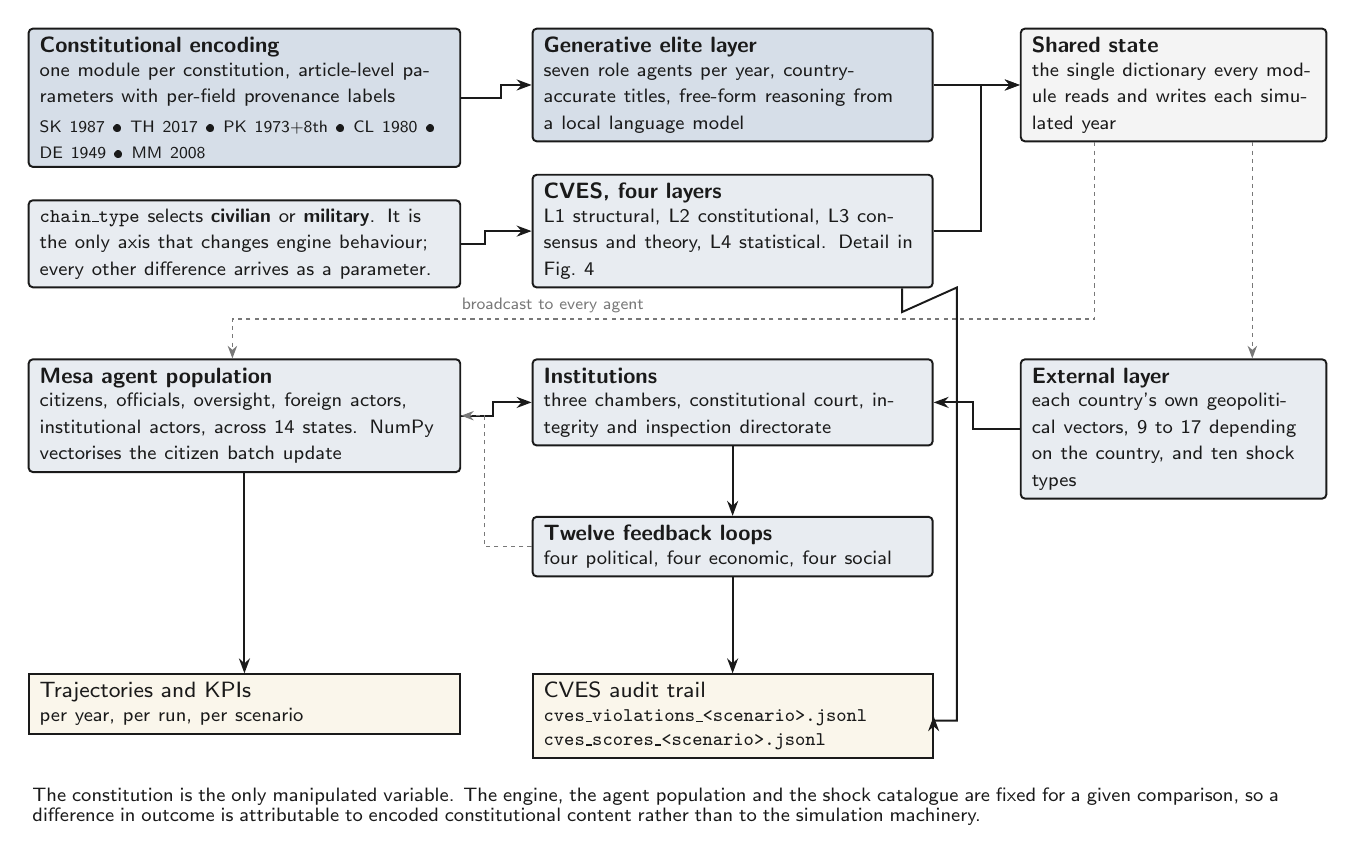
\begin{tikzpicture}[x=1mm, y=1mm]

\tikzset{
  N/.style={knbox, align=left, anchor=north west, minimum width=0pt},
  C/.style={knconst, align=left, anchor=north west, minimum width=0pt},
  F/.style={knfile, align=left, anchor=north west, minimum width=0pt},
}

% ===== constitutional layer ===============================================
\node[C, text width=52mm] (const) at (0,0)
  {\knhead{Constitutional encoding}\\[-1pt]\knsmall{one module per constitution,
   article-level parameters with per-field provenance labels}\\[1pt]
   \kntiny{SK 1987 \textbullet\ TH 2017 \textbullet\ PK 1973+8th \textbullet\
   CL 1980 \textbullet\ DE 1949 \textbullet\ MM 2008}};

\node[N, text width=52mm, below=4mm of const.south west, anchor=north west] (ctype)
  {\knsmall{\texttt{chain\_type} selects \textbf{civilian} or \textbf{military}.
   It is the only axis that changes engine behaviour; every other difference
   arrives as a parameter.}};

% ===== generative elite layer =============================================
\node[N, text width=48mm, fill=knfillC] (elite) at (64,0)
  {\knhead{Generative elite layer}\\[-1pt]\knsmall{seven role agents per year,
   country-accurate titles, free-form reasoning from a local language model}};

\node[N, text width=48mm, below=4mm of elite.south west, anchor=north west] (cves)
  {\knhead{CVES, four layers}\\[-1pt]\knsmall{L1 structural, L2 constitutional,
   L3 consensus and theory, L4 statistical. Detail in Fig.~4}};

% ===== shared state =======================================================
\node[N, text width=36mm, fill=knfillA] (bus) at (126,0)
  {\knhead{Shared state}\\[-1pt]\knsmall{the single dictionary every module
   reads and writes each simulated year}};

% ===== simulation core ====================================================
\node[N, text width=52mm] (agents) at (0,-42)
  {\knhead{Mesa agent population}\\[-1pt]\knsmall{citizens, officials,
   oversight, foreign actors, institutional actors, across 14 states.
   NumPy vectorises the citizen batch update}};

\node[N, text width=48mm] (inst) at (64,-42)
  {\knhead{Institutions}\\[-1pt]\knsmall{three chambers, constitutional court,
   integrity and inspection directorate}};

\node[N, text width=48mm] (fb) at (64,-62)
  {\knhead{Twelve feedback loops}\\[-1pt]\knsmall{four political, four
   economic, four social}};

\node[N, text width=36mm] (ext) at (126,-42)
  {\knhead{External layer}\\[-1pt]\knsmall{each country's own geopolitical
   vectors, 9 to 17 depending on the country, and ten shock types}};

% ===== outputs ============================================================
\node[F, text width=52mm] (out1) at (0,-82)
  {\knlabel{Trajectories and KPIs}\\[-1pt]\knsmall{per year, per run, per scenario}};
\node[F, text width=48mm] (out2) at (64,-82)
  {\knlabel{CVES audit trail}\\[-1pt]\kncode{cves\_violations\_<scenario>.jsonl}\\[-1pt]
   \kncode{cves\_scores\_<scenario>.jsonl}};

% ===== edges ==============================================================
\draw[knflow] (const.east) -- ++(5,0) |- (elite.west);
\draw[knflow] (ctype.east) -- ++(3,0) |- (cves.west);
\draw[knflow] (cves.east)  -- ++(6,0) |- (bus.west);
\draw[knflow] (elite.east) -- ++(6,0) |- (bus.west);

\draw[knread] ($(bus.south)+(10,0)$) -- ++(0,-6) -| ($(ext.north)+(10,0)$);
\draw[knflow] (ext.west)  -- ++(-6,0) |- (inst.east);
\draw[knflow] (agents.east) -- ++(4,0) |- (inst.west);
\draw[knflow] (inst.south) -- (fb.north);
\draw[knread] (fb.west) -- ++(-6,0) |- (agents.east);

% broadcast runs in the clear band between the upper and lower halves, so it
% crosses no box
\draw[knread] ($(bus.south)+(-10,0)$) |- (100,-37)
   -- node[knnote, pos=0.45, anchor=south, yshift=0.6] {broadcast to every agent}
   (26,-37) -- (26,-42);

\draw[knflow] (agents.south) -- (out1.north);
\draw[knflow] (fb.south)     -- ++(0,-4) -| (out2.north);
\draw[knflow] ($(cves.south east)+(-4,0)$) -- ++(0,-3) -- (118,-33) -- (118,-88)
   -- (out2.east |- 0,-88) -- (out2.east);

\node[knnote, anchor=north west, text width=160mm, text=knink] at (0,-96)
  {\knsmall{The constitution is the only manipulated variable. The engine,
  the agent population and the shock catalogue are fixed for a given
  comparison, so a difference in outcome is attributable to encoded
  constitutional content rather than to the simulation machinery.}};

\end{tikzpicture}
\end{document}
